\section{DiaTTS-Toolkit}
\subsection{Core Components}

\begin{frame}{DiaTTS-Toolkit}
  \setbeamercolor{caption}{bg=white}

  \setbeamertemplate{caption}{
    \begin{beamercolorbox}[wd=\linewidth, center, sep=2pt]{caption}
      {\usebeamercolor[fg]{caption name}\insertcaptionname:} \insertcaption
    \end{beamercolorbox}
  }
  \begin{figure}
    \vspace{-0.27cm}
    \centering
    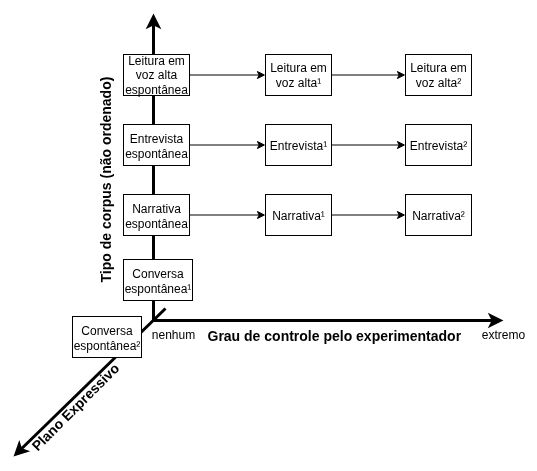
\includegraphics[width=0.5\linewidth]{imgs/DiaTTS-Toolkit-CorporaClasses.png}
    \tiny
    \caption{Classificação de \textit{córpora} segundo: grau de controle pelo
      experimentado; gênero enunciativo ; plano expressivo. Fonte: Adaptado de
    \citeauthor{Prosodia_Barbosa_2012} \cite{Prosodia_Barbosa_2012}.}
    \label{fig:corpora}
  \end{figure}
\end{frame}

\begin{frame}{DiaTTS-Toolkit}
  \setbeamercolor{caption}{bg=white}

  \setbeamertemplate{caption}{
    \begin{beamercolorbox}[wd=\linewidth, center, sep=2pt]{caption}
      {\usebeamercolor[fg]{caption name}\insertcaptionname:} \insertcaption
    \end{beamercolorbox}
  }

  \begin{figure}
    \centering
    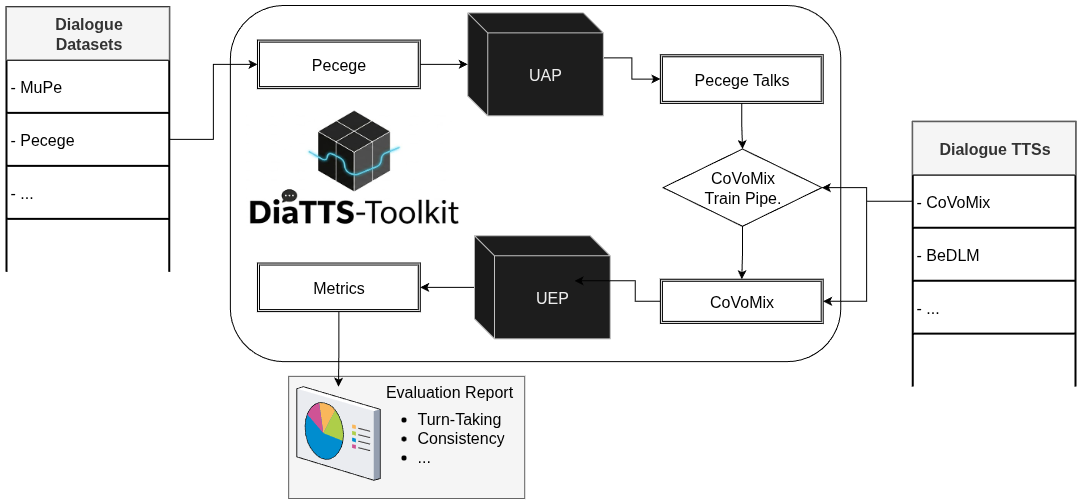
\includegraphics[width=1\linewidth]{imgs/DiaTTS-Toolkit-MainFlow.drawio.png}
    \caption{Esquemático \textit{DiaTTS-Toolkit}. Fonte: Elaborada pelo autor.}
    \label{fig:mainflow}
  \end{figure}
\end{frame}

\subsection{MuPeTalk}

\begin{frame}{MuPeTalk}
  \begin{block}{Pipeline de Criação}
    \begin{enumerate}
      \item Restrições do DailyTalk.
        \begin{itemize}
          \item $5+$ diálogos;
          \item Alternância de sexo;
        \end{itemize}
        \pause
      \item Restrição Adicional:
        \begin{itemize}
          \item Geográfica: Entrevistas \textit{apenas} de São Paulo capital;
        \end{itemize}
        \pause
      \item Inferência do sexo dos entrevistadores via
        \href{https://ai.google.dev/gemini-api/docs?hl=pt-br}{Gemini API}
    \end{enumerate}
  \end{block}
\end{frame}

\begin{frame}{MuPeTalk}
  \begin{figure}
    \centering
    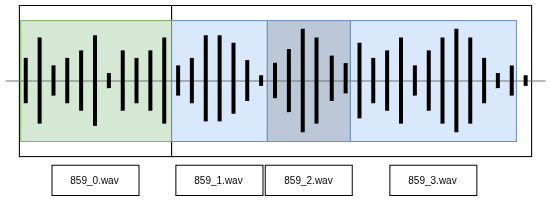
\includegraphics[width=1\linewidth]{imgs/MuPeTalk-MissingSegMuPe.drawio.png}
    \caption{Segmentos Faltantes}
    \label{fig:mupetalk}
  \end{figure}
\end{frame}

\subsection{PecegeTalk}

\begin{frame}{PecegeTalk}
  \begin{block}{}
    \begin{itemize}
      \item Pecege e Skylar
      \item Transcrição editada vs Transcrição Literal
    \end{itemize}
  \end{block}
\end{frame}

\begin{frame}{PecegeTalk}
  \begin{figure}
    \centering
    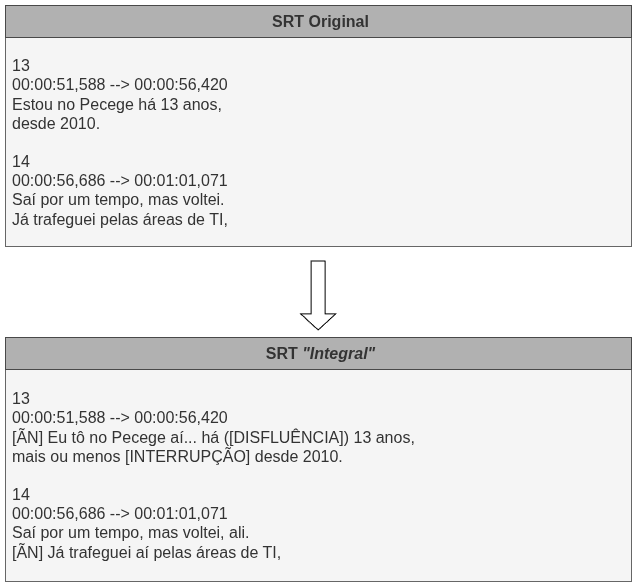
\includegraphics[width=0.6\linewidth]{imgs/MuPeTalk-PecegeTalk.drawio.png}
    \caption{\textbf{PecegeTalk}: Transcrição editada vs.\ Transcrição Literal}
    \label{fig:pecegetalk}
  \end{figure}
\end{frame}
